\chapter*{Markov Chain Monte Carlo}
\section{Introduction}
The application of probabilistic models to data often leads to inference problems that require the integration of complex, high dimensional distributions. Markov chain Monte Carlo (\textbf{MCMC}), is a general computational approach that replaces analytic integration by summation over samples generated from iterative algorithms.\\
Problems that are intractable using analytic approaches often become possible to solve using some form of \textbf{MCMC}, even with high-dimensional problems. \\
The development of \textbf{MCMC} is arguably the biggest advance in the computational approach to statistics. While \textbf{MCMC} is very much an active research area, there are now some standardized techniques that are widely used. In this chapter, after a brief introduction on the two main key ingredients of \textbf{MCMC} which are Monte Carlo integration and Markov chains, will discuss two forms of \textbf{MCMC}: \textit{Metropolis-Hastings} and \textit{Gibbs sampling}. 
\section{Monte Carlo Integration}
Many problems in probabilistic inference require the calculation of complex integrals or
summations over very large outcome spaces. For example, a frequent problem is to calculate
$E[g(x)]$,the expectation of a function $g(x)$ for the random variable $x$ (for simplicity, we assume $x$ is a univariate random variable) definde
If $x$ is continuous, the expectation is defined as:
\begin{eqnarray} \label{eqn: Expectation}
E[g(x)] = \left\{
\begin{array}{ccccc}
\int g(x)p(x)dx  & \mbox{if} & $x$ & is & continuous \\
\sum g(x)p(x)dx  & \mbox{if} & $x$ & is & discrete
\end{array}
\right.
\end{eqnarray}

These expectations arise in many situations where we want to calculate some statistic of a
distribution, such as the mean or variance. For example, if $g(x) = x$, we are calculating the mean of a distribution. Integration or summation using analytic techniques can become
quite challenging for certain distributions. For example, the density $p(x)$ might have a
functional form that does not lend itself to analytic integration. For discrete distributions, the outcome space might become so large to make the explicit summation over all possible outcomes impractical.\\
The general idea of Monte Carlo integration is to use samples to approximate the expectation of a complex distribution. Specifically, we obtain a set of samples $x(i), i = 1, . . . , N,$ drawn independently from distribution $p(x)$. In this case, we can approximate the expectations in \ref{eqn: Expectation} by a finite sum:
\begin{eqnarray} \label{eqn: Expectation Approx}
E[g(x)] = \sum_{i=1}^N g(x^i)p(x^i)
\end{eqnarray}
In this procedure, we have now replaced analytic integration with summation over a
suitably large set of samples. Generally, the accuracy of the approximation can be made as
accurate as needed by increasing $n$. Crucially, the precision of the approximation depends
on the independence of the samples: when the samples are correlated, the effective sample
size decreases.

\section{Markov Chain}
A Markov chain is a stochastic process where we transition from one state to another state
using a simple sequential procedure. We start a Markov chain at some state $x^1$, and use
a \textit{transition function} $p(x^t|x^{t-1})$, to determine the next state, $x^2$ conditioned on the last observed state. 
We then keep iterating to create a sequence of states:
$$
x^1  \rightarrow  x^2  \rightarrow . . . → x^t  \rightarrow . . .
$$
Each such a sequence of states is called a Markov chain or simply chain. The procedure
for generating a sequence of $T$ states from a Markov chain is the following:\\
{\bf MARKOV CHAIN GENERATION}\\[.4cm]
{\sf
0. \hspace*{0.2cm} Set $t=1$  \\
1. \hspace*{0.2cm} Generate a initial value $u$, and $set x^t = u$\\
3. \hspace*{0.2cm}  Repeat\\
3.1 \hspace*{0.3cm} $t=t+1$\\
3.2 \hspace*{0.3cm} Sample a new value $u$ from the transition function $p( x^t |x^{t-1})$\\
3.3 \hspace*{0.3cm} Set $x^t = u$\\
4. Until $t = T$\\
}\\[.4cm]
\\
\\


Importantly, in this iterative procedure, the next state of the chain at $t+1$ is based only on the previous state at t. Therefore, each Markov chain wanders around the state space and the transition to a new state is only dependent on the last state, giving to the whole procedure a \"memoryless\" property.
This local dependency behavior is an important property when using Markov chains for MCMC.
When initializing each Markov chain, the chain will wander in state space around the
starting state. Therefore, if we start a number of chains, each with different initial conditions, the chains will initially be in a state close to the starting state. This period is called the \textit{burnin}. An important property of Markov chains is that the starting state of the chain nolonger affects the state of the chain after a sufficiently long sequence of transitions (assuming that certain conditions about the Markov chain are met). At this point, the chain is said to reach its \textit{steady state} and the states reflect samples from its stationary distribution.
\\ This property that Markov chains converge to a stationary distribution regardless of where we started (if certain regularity conditions of the transition function are met), is quite important.
When applied to MCMC, it allow us to draw samples from a distribution using a sequential
procedure but where the starting state of the sequence does not affect the estimation process.
\newpage
\section{Markov chain Monte Carlo}
The two previous sections discussed the main two ideas underlying MCMC, Monte Carlo
sampling and Markov chains. Monte Carlo sampling allows one to estimate various characteristics of a distribution such as the mean, variance, kurtosis, or any other statistic of interest to a researcher. Markov chains involve a stochastic sequential process where we can sample states from some stationary distribution.\\
The goal of MCMC is to design a Markov chain such that the stationary distribution of
the chain is exactly the distribution that we are interesting in sampling from. This is called the \textit{target distribution}.\\
The target distribution could be the posterior distribution over the parameters in the model or the posterior predictive distribution of a model or any other distribution of interest to the researcher.\\
In other words, we would like the states sampled from some Markov chain to also be samples drawn from the target distribution. The idea is to use some clever methods for setting up the transition function such that no matter how we initialize each chain, we will convergence to the target distribution.\\
In the next section is discussed a general MCMC procedure and its modified version: Metropolis-Hastings and Metropolis.
\subsection{Metropolis sampler}
The Metropolis sampler is special case of the Metropolis-Hastings sampler discussed in the next section. Suppose our goal is to sample from the target density $p(\theta)$, with $-\inf < \theta < \inf$ . The Metropolis sampler creates a Markov chain that produces a sequence of states:
$$
\theta^1 \rightarrow  \theta^2 \rightarrow. . .  \rightarrow \theta^t  \rightarrow . . .
$$
where $\theta^t$ represents the state of a Markov chain at iteration $t$. 
The samples from the chain, after burnin, reflect samples from the target distribution $p(θ)$.\\
In the Metropolis procedure, we initialize the first state, $\theta^1$ to some initial value. We then use a proposal distribution $q(\theta^t|\theta^{t-1})$ to generate a candidate point $\theta^∗$ corresponding to a possible value for state at time $t$ conditioned on the previous state of the sampler. \\
The next step is to either accept the proposal or reject it. The probability $\alpha$ of accepting the proposal is definded as:\\
\begin{eqnarray} \label{eqn: Acceptance Ratio Metropolis}
\alpha = min(1, \frac{p(\theta^*)}{p(\theta^{t-1})})
\end{eqnarray}
To make a decision on whether to actually accept or reject the proposal, we generate a
uniform deviate $u$. If $u > \alpha$ , we accept the proposal and the next state is set equal to the proposal:  $\theta^t=\theta^{∗}$ . \\
 If $u \leq \alpha$, we reject the proposal, and the next state is set equal to the
old state: $\theta^t=\theta^{t-1}$ . We continue generating new proposals conditional on the current state of the sampler, and either accept or reject the proposals. This procedure continues until the sampler reaches convergence. At this point, the samples $\theta^t$ reflect samples from the target distribution $p(\theta)$. The Metropolis sampler algorithm is :\\
{\bf METROPOLIS Sampler}\\[.4cm]
{\sf
0. \hspace*{0.2cm} Set $t=1$  \\
1. \hspace*{0.2cm} Generate a initial value $u$, and $set x(t) = u$\\
2. \hspace*{0.2cm}  Repeat\\
2.1 \hspace*{0.3cm} $t=t+1$\\
2.2 \hspace*{0.3cm} generate a candidate point $\theta^∗$ from proposal distribution:
$$
\theta^∗ \approx q(\theta^t|\theta^{t-1}))
$$
2.3 \hspace*{0.3cm} calculate acceptance probability \\
$$
\alpha = min(1, \frac{p(\theta^*)}{p(\theta^{t-1})})
$$
2.4 \hspace*{0.3cm} generate $u$ from Uniform distribution in $[0 1]$\\
2.5 \hspace*{0.3cm} if($\alpha  \leq u$)\\
\hspace*{0.4cm}  \textbf{accept sample}: $\theta^t=\theta^∗$.\\
\hspace*{0.3cm} else\\
\hspace*{0.4cm}  \textbf{reject sample}: $\theta^t=\theta^{t-1}$.\\
3. \hspace*{0.2cm} Until $t = T$\\
}\\[.4cm]
\\
\\

\begin{figure}[!htb]
\begin{center}
\begin{tabular}{ccc}
 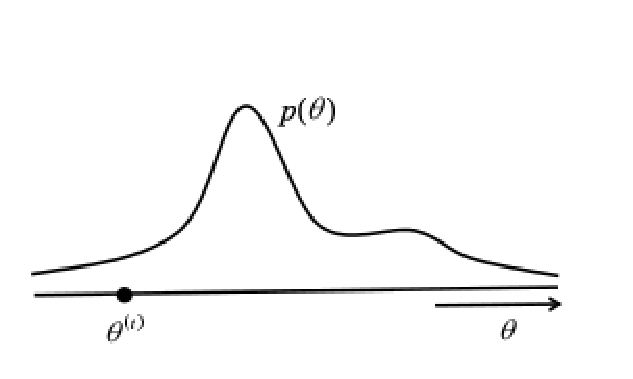
\includegraphics[width=4cm]{./ImaginiLatex/Metropolis1.eps} &
 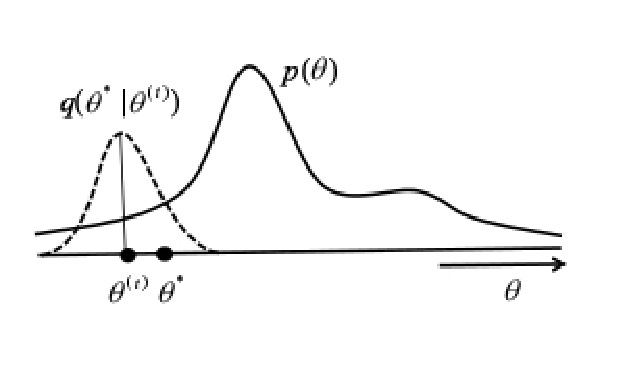
\includegraphics[width=4cm]{./ImaginiLatex/Metropolis2.eps} &
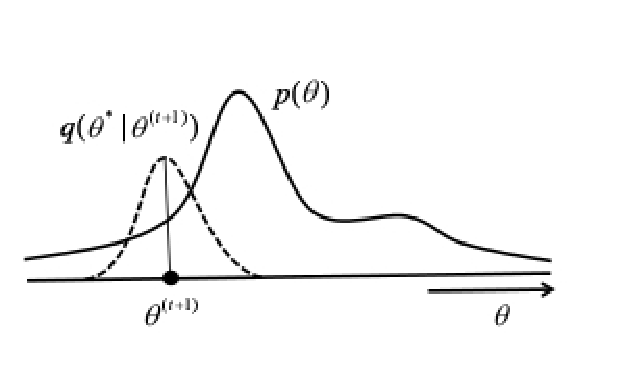
\includegraphics[width=4cm]{./ImaginiLatex/Metropolis3.eps} \\
a & b & c
\end{tabular}
\end{center}
\caption{Illustration of the Metropolis sampler to sample from target density $p(\theta)$. (a) the current state of the chain is $\theta^t$. (b) the proposal distribution $q$ around the current state is used to generate a proposal $\theta^*$ . 
(c) the proposal was accepted and the new state is set equal to the proposal, and the proposal distribution now centers on the new state.
 }
\label{fig:Metropolis}
\end{figure}

In Figure \ref{fig:Metropolis}  is illustrated how works the procedure for the generation of a sequence of two states. To intuitively understand why the process leads to samples from the target distribution, note that the method will always accept a new proposal if the the new proposal is more likely under the target distribution than the old state.
The proposal distribution is a distribution that is chosen by the researcher and good choices for the distribution depend on the problem. One important constraint for the proposal distribution is that it should cover the state space such that each potential outcome in state space has some non-zero probability under the proposal distribution 
old state. \\
Therefore, the sampler will move towards the regions of the state space where the target function has high density. However, note that if the new proposal is less likely than
than the current state, it is still possible to accept this "worse" proposal and move toward it. \\ This process of always accepting a "good" proposal, and occasionally accepting a "bad" proposal insures that the sampler explores the whole state space, and samples from all parts of a distribution (including the tails).\\
A key requirement for the Metropolis sampler is that the proposal distribution is symmetric, such that:
$$
q(\theta = \theta^t|\theta^{t-1} ) = q(\theta = \theta^{t-1} |\theta^t). 
$$
Therefore, the probability of proposing some new state given the old state, is the same as proposing to go from the new state back to the old state. This symmetry holds with proposal distributions such as the \textit{Normal, Cauchy, Student-t}, as well as \textit{Uniform} distributions. If this symmetry does not hold, you should use the Metropolis-Hastings sampler discussed in the next section.\\
A major advantage of the Metropolis sampler is that Equation \ref{eqn: Acceptance Ratio Metropolis} involves only a ratio of densities. Therefore, any terms independent of $\theta$ in the functional form of $p(\theta)$ will drop out.\\
Therefore, we do not need to know the normalizing constant of the density or probability mass function. The fact that this procedure allows us to sample from unnormalized distributions is one of its major attractions. Sampling from unnormalized distributions frequently happens in Bayesian models, where calculating the normalization constant is difficult or impractical.
\begin{example} \label{ex: Mixture of Gaussians Sampling}
In this example we try to generate random samples from a Mixture of Gaussians distribution given by:
$$
	p(\theta)=\sum_{i=1}^K \pi_i N_i(\theta | \mu_i,\sigma_i)
$$
where:
\begin{itemize}
\item $K$ is the number if components in the mixture;
\item $\pi_i$ are the mixing coefficients;
\item $N(\mu_i,\sigma_i)$ are the Gaussians components of the mixture.
\end{itemize}
Our proposals are generated from a Normal $N(\theta^t, \sigma)$ distribution. 
Therefore, the mean of the distribution is centered on the current state $\theta(t)$ and the parameter $\sigma$, which needs to be set by the modeler, controls the variability of the proposed samples.
We fixed $N=2$, $\pi=[0.3 0.5]$ , $N_1(\theta |5,4)$ , $N_2(\theta |30,3)$.
To explore the behavior of the sampling scheme we have generated different simulations varying the starting point $\theta(t_0)$ and  variability parameter $\sigma$, measuring the acceptance rate of the chain simulation.
\begin{figure}\label{fig: SimulationMetropolis0}
\begin{tabular}{cc} 
\includegraphics[width=0.5\textwidth]{ImaginiLatex/MetropolisExample1.eps} &
\includegraphics[width=0.5\textwidth]{ImaginiLatex/MetropolisExample2.eps} \\
\textbf{Simulation 1} $\theta_0=   95.33$  $\sigma=    0.25$  & \textbf{Simulation 2} $\theta_0=   70.70$  $\sigma=    0.50$
\end{tabular}
\begin{tabular}{cc} 
\includegraphics[width=0.5\textwidth]{ImaginiLatex/MetropolisExample3.eps} &
\includegraphics[width=0.5\textwidth]{ImaginiLatex/MetropolisExample4.eps} \\
\textbf{Simulation 3} $\theta_0=   95.43$  $\sigma=    0.75$  & \textbf{Simulation 4} $\theta_0=   60.22$  $\sigma=    1.00$
\end{tabular}
\begin{tabular}{cc} 
\includegraphics[width=0.5\textwidth]{ImaginiLatex/MetropolisExample5.eps} &
\includegraphics[width=0.5\textwidth]{ImaginiLatex/MetropolisExample6.eps} \\
\textbf{Simulation 5} $\theta_0=   84.23$  $\sigma=    1.25$  & \textbf{Simulation 6} $\theta_0=   44.84$  $\sigma=    1.50$
\end{tabular}
\begin{tabular}{cc} 
\includegraphics[width=0.5\textwidth]{ImaginiLatex/MetropolisExample7.eps} &
\includegraphics[width=0.5\textwidth]{ImaginiLatex/MetropolisExample8.eps} \\
\textbf{Simulation 7} $\theta_0=   83.85$  $\sigma=    1.75$  & \textbf{Simulation 8} $\theta_0=   52.35$  $\sigma=    2.00$
\end{tabular}
\caption{Simulations 1 - 8}
\end{figure}
\begin{figure}\label{fig: SimulationMetropolis1}
\begin{tabular}{cc} 
\includegraphics[width=0.5\textwidth]{ImaginiLatex/MetropolisExample9.eps} &
\includegraphics[width=0.5\textwidth]{ImaginiLatex/MetropolisExample10.eps} \\
\textbf{Simulation 9} $\theta_0=    3.20$  $\sigma=    2.25$  & \textbf{Simulation 10} $\theta_0=   38.21$  $\sigma=    2.50$
\end{tabular}
\begin{tabular}{cc} 
\includegraphics[width=0.5\textwidth]{ImaginiLatex/MetropolisExample11.eps} &
\includegraphics[width=0.5\textwidth]{ImaginiLatex/MetropolisExample12.eps} \\
\textbf{Simulation 11} $\theta_0=   89.96$  $\sigma=    2.75$  & \textbf{Simulation 12} $\theta_0=   43.47$  $\sigma=    3.00$
\end{tabular}
\begin{tabular}{cc} 
\includegraphics[width=0.5\textwidth]{ImaginiLatex/MetropolisExample13.eps} &
\includegraphics[width=0.5\textwidth]{ImaginiLatex/MetropolisExample14.eps} \\
\textbf{Simulation 13} $\theta_0=   20.76$  $\sigma=    3.25$  & \textbf{Simulation 14} $\theta_0=   31.01$  $\sigma=    3.50$
\end{tabular}
\begin{tabular}{cc} 
\includegraphics[width=0.5\textwidth]{ImaginiLatex/MetropolisExample15.eps} &
\includegraphics[width=0.5\textwidth]{ImaginiLatex/MetropolisExample16.eps} \\
\textbf{Simulation 15} $\theta_0=   54.29$  $\sigma=    3.75$  & \textbf{Simulation 16} $\theta_0=   91.11$  $\sigma=    4.00$
\end{tabular}
\caption{Simulations 2 - 16}
\end{figure}
\begin{figure}\label{fig: SimulationMetropolis2}
\begin{tabular}{cc} 
\includegraphics[width=0.5\textwidth]{ImaginiLatex/MetropolisExample17.eps} &
\includegraphics[width=0.5\textwidth]{ImaginiLatex/MetropolisExample18.eps} \\
\textbf{Simulation 17} $\theta_0=   53.00$  $\sigma=    4.25$  & \textbf{Simulation 18} $\theta_0=   31.38$  $\sigma=    4.50$
\end{tabular}
\begin{tabular}{cc} 
\includegraphics[width=0.5\textwidth]{ImaginiLatex/MetropolisExample19.eps} &
\includegraphics[width=0.5\textwidth]{ImaginiLatex/MetropolisExample20.eps} \\
\textbf{Simulation 19} $\theta_0=    4.41$  $\sigma=    4.75$  & \textbf{Simulation 20} $\theta_0=   71.82$  $\sigma=    5.00$
\end{tabular}
\begin{tabular}{cc} 
\includegraphics[width=0.5\textwidth]{ImaginiLatex/MetropolisExample21.eps} &
\includegraphics[width=0.5\textwidth]{ImaginiLatex/MetropolisExample22.eps} \\
\textbf{Simulation 21} $\theta_0=   77.10$  $\sigma=    5.25$  & \textbf{Simulation 22} $\theta_0=    6.89$  $\sigma=    5.50$
\end{tabular}
\begin{tabular}{cc} 
\includegraphics[width=0.5\textwidth]{ImaginiLatex/MetropolisExample23.eps} &
\includegraphics[width=0.5\textwidth]{ImaginiLatex/MetropolisExample24.eps} \\
\textbf{Simulation 23} $\theta_0=   63.08$  $\sigma=    5.75$  & \textbf{Simulation 24} $\theta_0=   27.25$  $\sigma=    6.00$
\end{tabular}
\caption{Simulations 3 - 24}
\end{figure}
\begin{figure}\label{fig: SimulationMetropolis3}
\begin{tabular}{cc} 
\includegraphics[width=0.5\textwidth]{ImaginiLatex/MetropolisExample25.eps} &
\includegraphics[width=0.5\textwidth]{ImaginiLatex/MetropolisExample26.eps} \\
\textbf{Simulation 25} $\theta_0=   31.92$  $\sigma=    6.25$  & \textbf{Simulation 26} $\theta_0=   52.75$  $\sigma=    6.50$
\end{tabular}
\begin{tabular}{cc} 
\includegraphics[width=0.5\textwidth]{ImaginiLatex/MetropolisExample27.eps} &
\includegraphics[width=0.5\textwidth]{ImaginiLatex/MetropolisExample28.eps} \\
\textbf{Simulation 27} $\theta_0=   41.45$  $\sigma=    6.75$  & \textbf{Simulation 28} $\theta_0=   89.40$  $\sigma=    7.00$
\end{tabular}
\begin{tabular}{cc} 
\includegraphics[width=0.5\textwidth]{ImaginiLatex/MetropolisExample29.eps} &
\includegraphics[width=0.5\textwidth]{ImaginiLatex/MetropolisExample30.eps} \\
\textbf{Simulation 29} $\theta_0=   57.80$  $\sigma=    7.25$  & \textbf{Simulation 30} $\theta_0=   57.22$  $\sigma=    7.50$
\end{tabular}
\begin{tabular}{cc} 
\includegraphics[width=0.5\textwidth]{ImaginiLatex/MetropolisExample31.eps} &
\includegraphics[width=0.5\textwidth]{ImaginiLatex/MetropolisExample32.eps} \\
\textbf{Simulation 31} $\theta_0=   40.06$  $\sigma=    7.75$  & \textbf{Simulation 32} $\theta_0=   69.47$  $\sigma=    8.00$
\end{tabular}
\caption{Simulations 4 - 32}
\end{figure}
\begin{figure}\label{fig: SimulationMetropolis4}
\begin{tabular}{cc} 
\includegraphics[width=0.5\textwidth]{ImaginiLatex/MetropolisExample33.eps} &
\includegraphics[width=0.5\textwidth]{ImaginiLatex/MetropolisExample34.eps} \\
\textbf{Simulation 33} $\theta_0=   57.36$  $\sigma=    8.25$  & \textbf{Simulation 34} $\theta_0=   34.98$  $\sigma=    8.50$
\end{tabular}
\begin{tabular}{cc} 
\includegraphics[width=0.5\textwidth]{ImaginiLatex/MetropolisExample35.eps} &
\includegraphics[width=0.5\textwidth]{ImaginiLatex/MetropolisExample36.eps} \\
\textbf{Simulation 35} $\theta_0=   59.90$  $\sigma=    8.75$  & \textbf{Simulation 36} $\theta_0=   28.12$  $\sigma=    9.00$
\end{tabular}
\end{figure}

Figure \ref{fig:SimulationMetropolis0} - \ref{fig:SimulationMetropolis4} show the simulation results for the different chains run for $500$ iterations.
The upper panel shows the theoretical density in the dashed red line and the histogram shows the distribution of all $500$ samples. The lower panel shows the sequence of samples of one chain.\\
Table \ref{tab: Simulation Metropolis} reports the acceptance ratio for each simulation.\\
\begin{center}
\begin{table}\label{tb: Simulation Metropolis}
\begin{tabular}{|ccccc|}\hline 
Simulation & $\theta_0$ & $\sigma$ & Acceptance ratio & Reject ratio)\\ \hline 
1 &    95.33 &     0.25 &     0.52 &     0.48 \\  \hline 
2 &    70.70 &     0.50 &     0.48 &     0.52 \\  
3 &    95.43 &     0.75 &     0.47 &     0.53 \\  
4 &    60.22 &     1.00 &     0.49 &     0.51 \\  
5 &    84.23 &     1.25 &     0.48 &     0.52 \\  
6 &    44.84 &     1.50 &     0.49 &     0.51 \\  
7 &    83.85 &     1.75 &     0.49 &     0.51 \\  
8 &    52.35 &     2.00 &     0.46 &     0.54 \\  
9 &     3.20 &     2.25 &     0.47 &     0.53 \\  
10 &    38.21 &     2.50 &     0.47 &     0.53 \\  
11 &    89.96 &     2.75 &     0.43 &     0.57 \\  
12 &    43.47 &     3.00 &     0.52 &     0.48 \\  
13 &    20.76 &     3.25 &     0.46 &     0.54 \\  
14 &    31.01 &     3.50 &     0.46 &     0.54 \\  
15 &    54.29 &     3.75 &     0.44 &     0.56 \\  
16 &    91.11 &     4.00 &     0.42 &     0.58 \\  
17 &    53.00 &     4.25 &     0.46 &     0.54 \\  
18 &    31.38 &     4.50 &     0.44 &     0.56 \\  
19 &     4.41 &     4.75 &     0.43 &     0.57 \\  
20 &    71.82 &     5.00 &     0.43 &     0.57 \\  
21 &    77.10 &     5.25 &     0.41 &     0.59 \\  
22 &     6.89 &     5.50 &     0.38 &     0.62 \\  
23 &    63.08 &     5.75 &     0.41 &     0.59 \\  
24 &    27.25 &     6.00 &     0.42 &     0.58 \\  
25 &    31.92 &     6.25 &     0.40 &     0.60 \\  
26 &    52.75 &     6.50 &     0.39 &     0.61 \\  
27 &    41.45 &     6.75 &     0.39 &     0.61 \\  
28 &    89.40 &     7.00 &     0.39 &     0.61 \\  
29 &    57.80 &     7.25 &     0.34 &     0.66 \\  
30 &    57.22 &     7.50 &     0.36 &     0.64 \\  
31 &    40.06 &     7.75 &     0.38 &     0.62 \\  
32 &    69.47 &     8.00 &     0.37 &     0.63 \\  
33 &    57.36 &     8.25 &     0.36 &     0.64 \\  
34 &    34.98 &     8.50 &     0.37 &     0.63 \\  
35 &    59.90 &     8.75 &     0.33 &     0.67 \\  
36 &    28.12 &     9.00 &     0.34 &     0.66 \\  
\end{tabular}
\caption{ Metropolis simulation results varying $\theta_0$ and $\sigma$ }
\end{table}
\end{center}



\end{example}

\newpage

\section{Metropolis-Hasting sampler}
The Metropolis-Hasting (\textbf{MH}) sampler is a generalized version of the Metropolis sampler in which we can apply symmetric as well as asymmetric proposal distributions. The \textbf{MH} sampler operates in exactly the same fashion as the Metropolis sampler, but uses the following acceptance probability: 
\begin{eqnarray} \label{eqn: Acceptance Ratio MH}
\alpha = min(1, \frac{p(\theta^*)}{p(\theta^{t-1})} \frac{q(\theta^{t-1}|\theta^∗) }{q(\theta^∗ |\theta^{t-1})}
\end{eqnarray}

The additional ratio $\frac{q(\theta^{t-1}|\theta^∗)}{q(\theta^∗ |\theta^{t-1})}$ in  \ref{eqn: Acceptance Ratio MH} corrects for any asymmetries in the proposal distribution. For example, suppose we have a proposal distribution with a mean centered on the current state, but that is skewed in one direction. If the proposal distribution prefers to move say left over right, the proposal density ratio will correct for this asymmetry.
We can summarize the \textbf{MH} sampler in the following operations:\\
{\bf METROPOLIS Sampler}\\[.4cm]
{\sf
0. \hspace*{0.2cm} Set $t=1$  \\
1. \hspace*{0.2cm} Generate a initial value $u$, and set $\theta^1 = u$\\
2. \hspace*{0.2cm}  Repeat\\
2.1 \hspace*{0.3cm} $t=t+1$\\
2.2 \hspace*{0.3cm} generate a candidate point $\theta^∗$ from proposal distribution:
$$
\theta^∗ \approx q(\theta^t |\theta^{t-1})
$$
2.3 \hspace*{0.3cm} calculate acceptance probability \\
$$
\alpha = min(1, \frac{p(\theta^*)}{p(\theta^{t-1})} \frac{q(\theta^{t-1}|\theta^∗)}{q(\theta^∗ |\theta^{t-1})} )
$$
2.4 \hspace*{0.3cm} generate $u$ from Uniform distribution in $[0 1]$\\
2.5 \hspace*{0.3cm} if($\alpha  \leq u$)\\
2.6 \hspace*{0.4cm}  \textbf{accept sample}: $\theta^t=\theta^∗$.\\
2.7 \hspace*{0.3cm} else\\
2.8 \hspace*{0.4cm}  \textbf{reject sample}: $\theta^t=\theta^{t-1}$.\\
3. \hspace*{0.2cm} Until $t = T$\\
}\\[.4cm]
\\
\\
The fact that asymmetric proposal distributions can be used allows the Metropolis-Hastings procedure to sample from target distributions that are defined on a limited range
(other than the uniform for which Metropolis sampler can be used). With bounded variables, care should be taken in constructing a suitable proposal distribution. Generally, a
good rule is to use a proposal distribution has positive density on the same support as the
target distribution.
\begin{example} \label{ex: Mixture of Gaussians Sampling 2}
In this example we try to generate random samples from the target distribution (\textbf{MOG}) discussed in example \ref{ex: Mixture of Gaussians Sampling}  using as proposal the Gamma distribution:
$$
q(\theta^t|\theta(t-1))= Gamma(\theta^t| \theta^{t-1} * \tau , frac{1}{\tau})
$$
This proposal density has a mean equal to $\theta^t$ so it is \"centered\" on the current state. The parameter $\tau$ is a precision parameter controlling the acceptance rate of the sampler so that higher values are associated with less variability in the proposal distribution.
\begin{figure}\label{fig: SimulationMetropolisHasting0}
\begin{tabular}{cc} 
\includegraphics[width=0.5\textwidth]{ImaginiLatex/MetropolisExample1.eps} &
\includegraphics[width=0.5\textwidth]{ImaginiLatex/MetropolisExample2.eps} \\
\textbf{Simulation 1} $\theta_0=   95.33$  $\tau=    0.25$  & \textbf{Simulation 2} $\theta_0=   70.70$  $\tau=    0.50$
\end{tabular}
\begin{tabular}{cc} 
\includegraphics[width=0.5\textwidth]{ImaginiLatex/MetropolisExample3.eps} &
\includegraphics[width=0.5\textwidth]{ImaginiLatex/MetropolisExample4.eps} \\
\textbf{Simulation 3} $\theta_0=   95.43$  $\tau=    0.75$  & \textbf{Simulation 4} $\theta_0=   60.22$  $\tau=    1.00$
\end{tabular}
\begin{tabular}{cc} 
\includegraphics[width=0.5\textwidth]{ImaginiLatex/MetropolisExample5.eps} &
\includegraphics[width=0.5\textwidth]{ImaginiLatex/MetropolisExample6.eps} \\
\textbf{Simulation 5} $\theta_0=   84.23$  $\tau=    1.25$  & \textbf{Simulation 6} $\theta_0=   44.84$  $\tau=    1.50$
\end{tabular}
\begin{tabular}{cc} 
\includegraphics[width=0.5\textwidth]{ImaginiLatex/MetropolisExample7.eps} &
\includegraphics[width=0.5\textwidth]{ImaginiLatex/MetropolisExample8.eps} \\
\textbf{Simulation 7} $\theta_0=   83.85$  $\tau=    1.75$  & \textbf{Simulation 8} $\theta_0=   52.35$  $\tau=    2.00$
\end{tabular}
\caption{Simulations 1 - 8}
\end{figure}
\begin{figure}\label{fig: SimulationMetropolisHasting1}
\begin{tabular}{cc} 
\includegraphics[width=0.5\textwidth]{ImaginiLatex/MetropolisExample9.eps} &
\includegraphics[width=0.5\textwidth]{ImaginiLatex/MetropolisExample10.eps} \\
\textbf{Simulation 9} $\theta_0=    3.20$  $\tau=    2.25$  & \textbf{Simulation 10} $\theta_0=   38.21$  $\tau=    2.50$
\end{tabular}
\begin{tabular}{cc} 
\includegraphics[width=0.5\textwidth]{ImaginiLatex/MetropolisExample11.eps} &
\includegraphics[width=0.5\textwidth]{ImaginiLatex/MetropolisExample12.eps} \\
\textbf{Simulation 11} $\theta_0=   89.96$  $\tau=    2.75$  & \textbf{Simulation 12} $\theta_0=   43.47$  $\tau=    3.00$
\end{tabular}
\begin{tabular}{cc} 
\includegraphics[width=0.5\textwidth]{ImaginiLatex/MetropolisExample13.eps} &
\includegraphics[width=0.5\textwidth]{ImaginiLatex/MetropolisExample14.eps} \\
\textbf{Simulation 13} $\theta_0=   20.76$  $\tau=    3.25$  & \textbf{Simulation 14} $\theta_0=   31.01$  $\tau=    3.50$
\end{tabular}
\begin{tabular}{cc} 
\includegraphics[width=0.5\textwidth]{ImaginiLatex/MetropolisExample15.eps} &
\includegraphics[width=0.5\textwidth]{ImaginiLatex/MetropolisExample16.eps} \\
\textbf{Simulation 15} $\theta_0=   54.29$  $\tau=    3.75$  & \textbf{Simulation 16} $\theta_0=   91.11$  $\tau=    4.00$
\end{tabular}
\caption{Simulations 2 - 16}
\end{figure}
\begin{figure}\label{fig: SimulationMetropolisHasting2}
\begin{tabular}{cc} 
\includegraphics[width=0.5\textwidth]{ImaginiLatex/MetropolisExample17.eps} &
\includegraphics[width=0.5\textwidth]{ImaginiLatex/MetropolisExample18.eps} \\
\textbf{Simulation 17} $\theta_0=   53.00$  $\tau=    4.25$  & \textbf{Simulation 18} $\theta_0=   31.38$  $\tau=    4.50$
\end{tabular}
\begin{tabular}{cc} 
\includegraphics[width=0.5\textwidth]{ImaginiLatex/MetropolisExample19.eps} &
\includegraphics[width=0.5\textwidth]{ImaginiLatex/MetropolisExample20.eps} \\
\textbf{Simulation 19} $\theta_0=    4.41$  $\tau=    4.75$  & \textbf{Simulation 20} $\theta_0=   71.82$  $\tau=    5.00$
\end{tabular}
\begin{tabular}{cc} 
\includegraphics[width=0.5\textwidth]{ImaginiLatex/MetropolisExample21.eps} &
\includegraphics[width=0.5\textwidth]{ImaginiLatex/MetropolisExample22.eps} \\
\textbf{Simulation 21} $\theta_0=   77.10$  $\tau=    5.25$  & \textbf{Simulation 22} $\theta_0=    6.89$  $\tau=    5.50$
\end{tabular}
\begin{tabular}{cc} 
\includegraphics[width=0.5\textwidth]{ImaginiLatex/MetropolisExample23.eps} &
\includegraphics[width=0.5\textwidth]{ImaginiLatex/MetropolisExample24.eps} \\
\textbf{Simulation 23} $\theta_0=   63.08$  $\tau=    5.75$  & \textbf{Simulation 24} $\theta_0=   27.25$  $\tau=    6.00$
\end{tabular}
\caption{Simulations 3 - 24}
\end{figure}
\begin{figure}\label{fig: SimulationMetropolisHasting3}
\begin{tabular}{cc} 
\includegraphics[width=0.5\textwidth]{ImaginiLatex/MetropolisExample25.eps} &
\includegraphics[width=0.5\textwidth]{ImaginiLatex/MetropolisExample26.eps} \\
\textbf{Simulation 25} $\theta_0=   31.92$  $\tau=    6.25$  & \textbf{Simulation 26} $\theta_0=   52.75$  $\tau=    6.50$
\end{tabular}
\begin{tabular}{cc} 
\includegraphics[width=0.5\textwidth]{ImaginiLatex/MetropolisExample27.eps} &
\includegraphics[width=0.5\textwidth]{ImaginiLatex/MetropolisExample28.eps} \\
\textbf{Simulation 27} $\theta_0=   41.45$  $\tau=    6.75$  & \textbf{Simulation 28} $\theta_0=   89.40$  $\tau=    7.00$
\end{tabular}
\begin{tabular}{cc} 
\includegraphics[width=0.5\textwidth]{ImaginiLatex/MetropolisExample29.eps} &
\includegraphics[width=0.5\textwidth]{ImaginiLatex/MetropolisExample30.eps} \\
\textbf{Simulation 29} $\theta_0=   57.80$  $\tau=    7.25$  & \textbf{Simulation 30} $\theta_0=   57.22$  $\tau=    7.50$
\end{tabular}
\begin{tabular}{cc} 
\includegraphics[width=0.5\textwidth]{ImaginiLatex/MetropolisExample31.eps} &
\includegraphics[width=0.5\textwidth]{ImaginiLatex/MetropolisExample32.eps} \\
\textbf{Simulation 31} $\theta_0=   40.06$  $\tau=    7.75$  & \textbf{Simulation 32} $\theta_0=   69.47$  $\tau=    8.00$
\end{tabular}
\caption{Simulations 4 - 32}
\end{figure}
\begin{figure}\label{fig: SimulationMetropolisHasting4}
\begin{tabular}{cc} 
\includegraphics[width=0.5\textwidth]{ImaginiLatex/MetropolisExample33.eps} &
\includegraphics[width=0.5\textwidth]{ImaginiLatex/MetropolisExample34.eps} \\
\textbf{Simulation 33} $\theta_0=   57.36$  $\tau=    8.25$  & \textbf{Simulation 34} $\theta_0=   34.98$  $\tau=    8.50$
\end{tabular}
\begin{tabular}{cc} 
\includegraphics[width=0.5\textwidth]{ImaginiLatex/MetropolisExample35.eps} &
\includegraphics[width=0.5\textwidth]{ImaginiLatex/MetropolisExample36.eps} \\
\textbf{Simulation 35} $\theta_0=   59.90$  $\tau=    8.75$  & \textbf{Simulation 36} $\theta_0=   28.12$  $\tau=    9.00$
\end{tabular}
\end{figure}

In figures \ref{fig:SimulationMetropolisHasting0} - \ref{fig:SimulationMetropolisHasting4} are depicted the simulation results for different chains runs for $500$ iterations.
Again, in the upper panel are depicted the theoretical density in the dashed red line and the distribution of all $500$ generated samples, while in the lower panel is showed the sequence in time of generated samples (rejected and accepted samples).\\
In table ~\ref{tab: Simulation Metropolis} we report the acceptance ratio for each simulation.\\
\begin{center}
\begin{table}\label{tb: Simulation Metropolis}
\begin{tabular}{|ccccc|}\hline 
Simulation & $\theta_0$ & $\sigma$ & Acceptance ratio & Reject ratio)\\ \hline 
1 &    95.33 &     0.25 &     0.38 &     0.62 \\  \hline 
2 &    70.70 &     0.50 &     0.42 &     0.58 \\  
3 &    95.43 &     0.75 &     0.47 &     0.53 \\  
4 &    60.22 &     1.00 &     0.53 &     0.47 \\  
5 &    84.23 &     1.25 &     0.51 &     0.49 \\  
6 &    44.84 &     1.50 &     0.50 &     0.50 \\  
7 &    83.85 &     1.75 &     0.61 &     0.39 \\  
8 &    52.35 &     2.00 &     0.60 &     0.40 \\  
9 &     3.20 &     2.25 &     0.61 &     0.39 \\  
10 &    38.21 &     2.50 &     0.61 &     0.39 \\  
11 &    89.96 &     2.75 &     0.66 &     0.34 \\  
12 &    43.47 &     3.00 &     0.70 &     0.30 \\  
13 &    20.76 &     3.25 &     0.73 &     0.27 \\  
14 &    31.01 &     3.50 &     0.64 &     0.36 \\  
15 &    54.29 &     3.75 &     0.70 &     0.30 \\  
16 &    91.11 &     4.00 &     0.69 &     0.31 \\  
17 &    53.00 &     4.25 &     0.73 &     0.27 \\  
18 &    31.38 &     4.50 &     0.78 &     0.22 \\  
19 &     4.41 &     4.75 &     0.72 &     0.28 \\  
20 &    71.82 &     5.00 &     0.71 &     0.29 \\  
21 &    77.10 &     5.25 &     0.74 &     0.26 \\  
22 &     6.89 &     5.50 &     0.71 &     0.29 \\  
23 &    63.08 &     5.75 &     0.76 &     0.24 \\  
24 &    27.25 &     6.00 &     0.75 &     0.25 \\  
25 &    31.92 &     6.25 &     0.80 &     0.20 \\  
26 &    52.75 &     6.50 &     0.75 &     0.25 \\  
27 &    41.45 &     6.75 &     0.71 &     0.29 \\  
28 &    89.40 &     7.00 &     0.71 &     0.29 \\  
29 &    57.80 &     7.25 &     0.77 &     0.23 \\  
30 &    57.22 &     7.50 &     0.70 &     0.30 \\  
31 &    40.06 &     7.75 &     0.80 &     0.20 \\  
32 &    69.47 &     8.00 &     0.72 &     0.28 \\  
33 &    57.36 &     8.25 &     0.74 &     0.26 \\  
34 &    34.98 &     8.50 &     0.79 &     0.21 \\  
35 &    59.90 &     8.75 &     0.76 &     0.24 \\  
36 &    28.12 &     9.00 &     0.88 &     0.12 \\  
\end{tabular}
\caption{ Metropolis simulation results varying $\theta_0$ and $\sigma$ }
\end{table}
\end{center}

\end{example}
\newpage
\subsection{Metropolis-Hastings for Multivariate Distributions}
The generalization of MH sampler to multivariate distributions can be obtained following two different approaches differing each other in the strategy used to explore multidimensional spaces, namely blockwise or componentwise upadating.
Let $\mathbf{\theta} = (\theta_1, \theta_2 , . . . ,\theta_N )$ be a random variable involving $N$ components, our objective is to generate a chain:
$$
\mathbf{\theta^1}  \rightarrow  \mathbf{\theta^2}  \rightarrow . .  \rightarrow  \mathbf{\theta^t}  \rightarrow . . .
$$
where  $\mathbf{\theta^t}$ represents the N-dimensional sample generated at time $t$.

\subsubsection{Blockwise updating}
The blockwise updating approach uses a proposal distribution having same dimensionality as the target distribution. So, if we want to sample from a probability distribution involving $N$ variables, we design a N-dimensional proposal distribution, and we either accept or reject the proposal (involving values for all $N$ variables) as a block.\\
This leads to a generalization of the \textbf{MH} sampler where the scalar samples $\theta^t$ are now replaced by vectors $\mathbf{\theta^t}$:\\
{\bf METROPOLIS HASTING B.W}\\[.4cm]
{\sf
0. \hspace*{0.2cm} Set $t=1$  \\
1. \hspace*{0.2cm} Generate a initial value $\mathbf{\theta^1}=(\theta_1^1, \theta_2^1 , . . . ,\theta_N^1 )$\
2. \hspace*{0.2cm}  Repeat\\
2.1 \hspace*{0.3cm} $t=t+1$\\
2.2 \hspace*{0.3cm} generate a candidate point $\theta^∗$ from proposal distribution:\\
$$
\mathbf{\theta^∗} \approx q(\mathbf{\theta^t}|\mathbf{ \theta^{t-1} })
$$
2.3 \hspace*{0.3cm} calculate acceptance probability \\
$$
\alpha = min(1, \frac{p(\mathbf{\theta^*})}{p(\mathbf{\theta^{t-1}})} \frac{q(\mathbf{\theta^{t-1}}|\mathbf{\theta^∗})}{q(\mathbf{\theta^∗} |\mathbf{\theta^{t-1}})} )
$$
2.4 \hspace*{0.3cm} generate $u$ from Uniform distribution in $[0 1]$\\
2.5 \hspace*{0.3cm} if($\alpha  \leq u$)\\
\hspace*{0.4cm}  \textbf{accept sample}: $\theta^t=\theta^∗$.\\
\hspace*{0.3cm} else\\
\hspace*{0.4cm}  \textbf{reject sample}: $\theta^t=\theta^{t-1}$.\\
3. \hspace*{0.2cm} Until $t = T$\\
}\\[.4cm]
\\
\\
A potential problem with the blockwise updating approach is that it might be difficult to
find suitable high-dimensional proposal distributions. A related problem is that blockwise
updating can be associated with high rejection rates. 
\subsubsection{Componentwise updating}
Instead of accepting or rejecting a proposal for $\theta$ involving all its components simultaneously, the component wise approach generate proposal for individual components of $\theta$, once per time.\\
This leads to a  computationally simpler updating approach where at each iteration $t$, we  make an independent proposal $\theta_i^*$ for each component status $\theta_i^t$ given its previous state  $\theta_i^{t-1}$ and evaluate the acceptance ratio comparing the likelihood of $(\theta_i^* , \theta_{j\neq i}^{t-1} )$ against $(\theta_i^{t-1} , \theta_{j\neq i}^{t-1} )$.
Note that in this proposal procedure, we  vary at each time only one component keeping the others component constant and updated to the last generated proposal.  Therefore, what happens while proposing a new sample for $\theta_{j}^{t}$ is conditioned on what
happened in proposal generation for all components $i<j$ .
The whole procedure is summarized in the following steps:\\

{\bf METROPOLIS-HASTING C.W. }\\[.4cm]
{\sf
0. \hspace*{0.2cm} Set $t=1$  \\
1. \hspace*{0.2cm} Generate a initial value $\mathbf{\theta^1}=(\theta_1^1, \theta_2^1 , . . . ,\theta_N^1 )$\\
2. \hspace*{0.2cm}  Repeat\\
2.1 \hspace*{0.3cm} $t=t+1$\\
2.2 \hspace*{0.3cm}  For $i=1:N$\\
2.2 \hspace*{0.4cm} generate a candidate component $\theta_i^∗$ from proposal distribution:
$$
\theta_i^∗ \approx q( \theta_i^t |\theta_i^{t-1} )
$$
3.3 \hspace*{0.4cm} calculate acceptance probability \\
$$
\alpha = min(1, \frac{p(\theta_i^*,\theta_{j \neq i}^{t-1})}{p(\mathbf{\theta^{t-1}})} \frac{q( \theta_i^{t-1}| \theta_i^{∗} ) } { q( \theta_i^{∗}| \theta_i^{t-1} )} )
$$
2.4 \hspace*{0.4cm} generate $u$ from Uniform distribution in $[0 1]$\\
2.4 \hspace*{0.4cm} if($\alpha  \leq u$)\\
2.5 \hspace*{0.5cm}  \textbf{accept sample component}: $\theta_i^t=\theta_i^∗$.\\
2.6 \hspace*{0.4cm} else\\
2.7 \hspace*{0.5cm}  \textbf{reject sample component}: $\theta_i^t=\theta_i^{t-1}$.\\
2.8 \hspace*{0.3cm}  EndFor \\
3.\hspace*{0.2cm} Until $t = T$\\
}\\[.4cm]
\\
\\
\begin{example} \label{ex: Mixture of Multivariate Gaussians Sampling}
In this example we try to generate random samples from a Mixture of multivariate Gaussians distribution given by:
$$
	p(\theta)=\sum_{i=1}^K \pi(i)N_i(\theta | \mu_i,\Sigma_i)
$$
where:
\begin{itemize}
\item $K$ is the number if components in the mixture;
\item $\pi_i$ are the mixing coefficients;
\item $N(\mu_i,\Sigma_i)$ are the multivariate Gaussians components of the mixture 
parametrized by the mean vector $1 \times N \mu$ and the covariance matrix
$N \times N \Sigma$
\end{itemize}
We used as proposal the Gamma distribution described in \ref{ex: Mixture of Gaussians Sampling 2}
We fixed $N=2$, $\pi=[0.3 0.5]$ , $N_1(\theta |5,4)$ , $N_2(\theta |30,3)$.
To explore the behavior of the sampling scheme we have generated different simulations varying the starting point $\theta(t_0)$ and the Gamma distribution parameters , measuring the acceptance rate of each chain simulation. In table ~\ref{tab: Simulation Metropolis} are reported obtained result.
\begin{center}
\begin{table}\label{tb: Simulation Metropolis}
\begin{tabular}{|cccccc|}\hline 
Simulation & $\theta_0$ & $a$ & $b$ & Acceptance ratio & Reject ratio)\\ \hline 
1 & (    5.00 ,     5.00) &     0.10 &     1.00 &     1.00 &     0.00 \\  \hline\hline 
2 & (    5.00 ,     5.00) &     0.10 &     2.00 &     0.98 &     0.02 \\  \hline
3 & (    5.00 ,     5.00) &     0.10 &     3.00 &     1.00 &     0.00 \\  \hline
4 & (    5.00 ,     5.00) &     0.10 &     4.00 &     0.77 &     0.23 \\  \hline
5 & (    5.00 ,     5.00) &     0.57 &     1.00 &     0.92 &     0.08 \\  \hline
6 & (    5.00 ,     5.00) &     0.57 &     2.00 &     0.38 &     0.62 \\  \hline
7 & (    5.00 ,     5.00) &     0.57 &     3.00 &     0.08 &     0.92 \\  \hline
8 & (    5.00 ,     5.00) &     0.57 &     4.00 &     0.01 &     0.99 \\  \hline
9 & (    5.00 ,     5.00) &     1.03 &     2.00 &     0.01 &     0.99 \\  \hline
10 & (    5.00 ,     5.00) &     1.03 &     3.00 &     0.00 &     1.00 \\  \hline
11 & (    5.00 ,     5.00) &     1.03 &     4.00 &     0.00 &     1.00 \\  \hline
12 & (    5.00 ,     5.00) &     1.50 &     2.00 &     0.00 &     1.00 \\  \hline
13 & (    5.00 ,     5.00) &     1.50 &     3.00 &     0.94 &     0.06 \\  \hline
14 & (    5.00 ,     5.00) &     1.50 &     4.00 &     1.00 &     0.00 \\  \hline
15 & (   11.67 ,    11.67) &     0.10 &     1.00 &     1.00 &     0.00 \\  \hline
16 & (   11.67 ,    11.67) &     0.10 &     2.00 &     0.94 &     0.06 \\  \hline
17 & (   11.67 ,    11.67) &     0.10 &     3.00 &     0.97 &     0.03 \\  \hline
18 & (   11.67 ,    11.67) &     0.10 &     4.00 &     0.73 &     0.27 \\  \hline
19 & (   11.67 ,    11.67) &     0.57 &     1.00 &     0.97 &     0.03 \\  \hline
20 & (   11.67 ,    11.67) &     0.57 &     2.00 &     0.41 &     0.59 \\  \hline
21 & (   11.67 ,    11.67) &     0.57 &     3.00 &     0.05 &     0.95 \\  \hline
22 & (   11.67 ,    11.67) &     0.57 &     4.00 &     0.01 &     0.99 \\  \hline
23 & (   11.67 ,    11.67) &     1.03 &     2.00 &     0.00 &     1.00 \\  \hline
24 & (   11.67 ,    11.67) &     1.03 &     3.00 &     0.00 &     1.00 \\  \hline
25 & (   11.67 ,    11.67) &     1.03 &     4.00 &     0.00 &     1.00 \\  \hline
26 & (   11.67 ,    11.67) &     1.50 &     2.00 &     0.00 &     1.00 \\  \hline
27 & (   11.67 ,    11.67) &     1.50 &     3.00 &     0.98 &     0.02 \\  \hline
28 & (   11.67 ,    11.67) &     1.50 &     4.00 &     0.99 &     0.01 \\  \hline
29 & (   18.33 ,    18.33) &     0.10 &     1.00 &     1.00 &     0.00 \\  \hline
30 & (   18.33 ,    18.33) &     0.10 &     2.00 &     0.97 &     0.03 \\  \hline
31 & (   18.33 ,    18.33) &     0.10 &     3.00 &     0.94 &     0.06 \\  \hline
32 & (   18.33 ,    18.33) &     0.10 &     4.00 &     0.82 &     0.18 \\  \hline
33 & (   18.33 ,    18.33) &     0.57 &     1.00 &     0.95 &     0.05 \\  \hline
34 & (   18.33 ,    18.33) &     0.57 &     2.00 &     0.40 &     0.60 \\  \hline
35 & (   18.33 ,    18.33) &     0.57 &     3.00 &     0.06 &     0.94 \\  \hline
36 & (   18.33 ,    18.33) &     0.57 &     4.00 &     0.01 &     0.99 \\  \hline
37 & (   18.33 ,    18.33) &     1.03 &     2.00 &     0.00 &     1.00 \\  \hline
38 & (   18.33 ,    18.33) &     1.03 &     3.00 &     0.00 &     1.00 \\  \hline
39 & (   18.33 ,    18.33) &     1.03 &     4.00 &     0.00 &     1.00 \\  \hline
40 & (   18.33 ,    18.33) &     1.50 &     2.00 &     0.00 &     1.00 \\  \hline
41 & (   18.33 ,    18.33) &     1.50 &     3.00 &     0.46 &     0.54 \\  \hline
42 & (   18.33 ,    18.33) &     1.50 &     4.00 &     0.93 &     0.07 \\  \hline
43 & (   25.00 ,    25.00) &     0.10 &     1.00 &     0.99 &     0.01 \\  \hline
44 & (   25.00 ,    25.00) &     0.10 &     2.00 &     0.97 &     0.03 \\  \hline
45 & (   25.00 ,    25.00) &     0.10 &     3.00 &     0.97 &     0.03 \\  \hline
46 & (   25.00 ,    25.00) &     0.10 &     4.00 &     0.98 &     0.02 \\  \hline
47 & (   25.00 ,    25.00) &     0.57 &     1.00 &     0.95 &     0.05 \\  \hline
48 & (   25.00 ,    25.00) &     0.57 &     2.00 &     0.37 &     0.63 \\  \hline
49 & (   25.00 ,    25.00) &     0.57 &     3.00 &     0.07 &     0.94 \\  \hline
50 & (   25.00 ,    25.00) &     0.57 &     4.00 &     0.01 &     0.99 \\  \hline
51 & (   25.00 ,    25.00) &     1.03 &     2.00 &     0.00 &     1.00 \\  \hline
52 & (   25.00 ,    25.00) &     1.03 &     3.00 &     0.00 &     1.00 \\  \hline
53 & (   25.00 ,    25.00) &     1.03 &     4.00 &     0.00 &     1.00 \\  \hline
54 & (   25.00 ,    25.00) &     1.50 &     2.00 &     0.00 &     1.00 \\  \hline
55 & (   25.00 ,    25.00) &     1.50 &     3.00 &     0.00 &     1.00 \\  \hline
56 & (   25.00 ,    25.00) &     1.50 &     4.00 &     0.98 &     0.02 \\  \hline
\end{tabular}
\caption{ Metropolis simulation results varying $\theta_0$ and $\sigma$ }
\end{table}
\end{center}

Reported results underline a typical drawback of the Metropolis-Hastings scheme and in general of rejection samplers: the difficulties
in tuning the proposal distribution to avoid production of rejected samples that are no used in approximation process. 
In figures \ref{fig:SimulationMetropolisHasting0} - \ref{fig:SimulationMetropolisHasting4} are showed the simulation results for different chains runs for $500$ iterations:  in the upper panel is depicted the histogram of generated samples, while in the lower panel are showed the isolines of the sampled distribution and the sequence of generated samples . The green point correspond to the starting sample, the blue point is the last generated sample while the red ones are samples generated during the simulation.\\
Again, the simulation shows how could be difficult to tune the proposal distribution.
\centering
\begin{figure}\label{fig: SimulationMetropolisHasting0}
\begin{tabular}{cc} 
\includegraphics[width=0.5\textwidth]{ImaginiLatex/MetropolisHastingCWExample1.eps} &
\includegraphics[width=0.5\textwidth]{ImaginiLatex/MetropolisHastingCWExample2.eps} \\
\textbf{Simulation 1} $\theta_0=(    5.00,     5.00)$  $(a,b)=(    0.10,    1.00)$  & \textbf{Simulation 2} $\theta_0=(    5.00,     5.00)$  $(a,b)=(    0.10,    2.00)$
\end{tabular}
\begin{tabular}{cc} 
\includegraphics[width=0.5\textwidth]{ImaginiLatex/MetropolisHastingCWExample3.eps} &
\includegraphics[width=0.5\textwidth]{ImaginiLatex/MetropolisHastingCWExample4.eps} \\
\textbf{Simulation 3} $\theta_0=(    5.00,     5.00)$  $(a,b)=(    0.10,    3.00)$  & \textbf{Simulation 4} $\theta_0=(    5.00,     5.00)$  $(a,b)=(    0.10,    4.00)$
\end{tabular}
\begin{tabular}{cc} 
\includegraphics[width=0.5\textwidth]{ImaginiLatex/MetropolisHastingCWExample5.eps} &
\includegraphics[width=0.5\textwidth]{ImaginiLatex/MetropolisHastingCWExample6.eps} \\
\textbf{Simulation 5} $\theta_0=(    5.00,     5.00)$  $(a,b)=(    0.57,    1.00)$  & \textbf{Simulation 6} $\theta_0=(    5.00,     5.00)$  $(a,b)=(    0.57,    2.00)$
\end{tabular}
\begin{tabular}{cc} 
\includegraphics[width=0.5\textwidth]{ImaginiLatex/MetropolisHastingCWExample7.eps} &
\includegraphics[width=0.5\textwidth]{ImaginiLatex/MetropolisHastingCWExample8.eps} \\
\textbf{Simulation 7} $\theta_0=(    5.00,     5.00)$  $(a,b)=(    0.57,    3.00)$  & \textbf{Simulation 8} $\theta_0=(    5.00,     5.00)$  $(a,b)=(    0.57,    4.00)$
\end{tabular}
\caption{Simulations 1 - 8}
\end{figure}
\begin{figure}\label{fig: SimulationMetropolisHastingCW1}
\begin{tabular}{cc} 
\includegraphics[width=0.5\textwidth]{ImaginiLatex/MetropolisHastingCWExample9.eps} &
\includegraphics[width=0.5\textwidth]{ImaginiLatex/MetropolisHastingCWExample10.eps} \\
\textbf{Simulation 9} $\theta_0=(    5.00,     5.00)$  $(a,b)=(    1.03,    2.00)$  & \textbf{Simulation 10} $\theta_0=(    5.00,     5.00)$  $(a,b)=(    1.03,    3.00)$
\end{tabular}
\begin{tabular}{cc} 
\includegraphics[width=0.5\textwidth]{ImaginiLatex/MetropolisHastingCWExample11.eps} &
\includegraphics[width=0.5\textwidth]{ImaginiLatex/MetropolisHastingCWExample12.eps} \\
\textbf{Simulation 11} $\theta_0=(    5.00,     5.00)$  $(a,b)=(    1.03,    4.00)$  & \textbf{Simulation 12} $\theta_0=(    5.00,     5.00)$  $(a,b)=(    1.50,    2.00)$
\end{tabular}
\begin{tabular}{cc} 
\includegraphics[width=0.5\textwidth]{ImaginiLatex/MetropolisHastingCWExample13.eps} &
\includegraphics[width=0.5\textwidth]{ImaginiLatex/MetropolisHastingCWExample14.eps} \\
\textbf{Simulation 13} $\theta_0=(    5.00,     5.00)$  $(a,b)=(    1.50,    3.00)$  & \textbf{Simulation 14} $\theta_0=(    5.00,     5.00)$  $(a,b)=(    1.50,    4.00)$
\end{tabular}
\begin{tabular}{cc} 
\includegraphics[width=0.5\textwidth]{ImaginiLatex/MetropolisHastingCWExample15.eps} &
\includegraphics[width=0.5\textwidth]{ImaginiLatex/MetropolisHastingCWExample16.eps} \\
\textbf{Simulation 15} $\theta_0=(   11.67,    11.67)$  $(a,b)=(    0.10,    1.00)$  & \textbf{Simulation 16} $\theta_0=(   11.67,    11.67)$  $(a,b)=(    0.10,    2.00)$
\end{tabular}
\caption{Simulations 2 - 16}
\end{figure}
\begin{figure}\label{fig: SimulationMetropolisHastingCW2}
\begin{tabular}{cc} 
\includegraphics[width=0.5\textwidth]{ImaginiLatex/MetropolisHastingCWExample17.eps} &
\includegraphics[width=0.5\textwidth]{ImaginiLatex/MetropolisHastingCWExample18.eps} \\
\textbf{Simulation 17} $\theta_0=(   11.67,    11.67)$  $(a,b)=(    0.10,    3.00)$  & \textbf{Simulation 18} $\theta_0=(   11.67,    11.67)$  $(a,b)=(    0.10,    4.00)$
\end{tabular}
\begin{tabular}{cc} 
\includegraphics[width=0.5\textwidth]{ImaginiLatex/MetropolisHastingCWExample19.eps} &
\includegraphics[width=0.5\textwidth]{ImaginiLatex/MetropolisHastingCWExample20.eps} \\
\textbf{Simulation 19} $\theta_0=(   11.67,    11.67)$  $(a,b)=(    0.57,    1.00)$  & \textbf{Simulation 20} $\theta_0=(   11.67,    11.67)$  $(a,b)=(    0.57,    2.00)$
\end{tabular}
\begin{tabular}{cc} 
\includegraphics[width=0.5\textwidth]{ImaginiLatex/MetropolisHastingCWExample21.eps} &
\includegraphics[width=0.5\textwidth]{ImaginiLatex/MetropolisHastingCWExample22.eps} \\
\textbf{Simulation 21} $\theta_0=(   11.67,    11.67)$  $(a,b)=(    0.57,    3.00)$  & \textbf{Simulation 22} $\theta_0=(   11.67,    11.67)$  $(a,b)=(    0.57,    4.00)$
\end{tabular}
\begin{tabular}{cc} 
\includegraphics[width=0.5\textwidth]{ImaginiLatex/MetropolisHastingCWExample23.eps} &
\includegraphics[width=0.5\textwidth]{ImaginiLatex/MetropolisHastingCWExample24.eps} \\
\textbf{Simulation 23} $\theta_0=(   11.67,    11.67)$  $(a,b)=(    1.03,    2.00)$  & \textbf{Simulation 24} $\theta_0=(   11.67,    11.67)$  $(a,b)=(    1.03,    3.00)$
\end{tabular}
\caption{Simulations 3 - 24}
\end{figure}
\begin{figure}\label{fig: SimulationMetropolisHastingCW3}
\begin{tabular}{cc} 
\includegraphics[width=0.5\textwidth]{ImaginiLatex/MetropolisHastingCWExample25.eps} &
\includegraphics[width=0.5\textwidth]{ImaginiLatex/MetropolisHastingCWExample26.eps} \\
\textbf{Simulation 25} $\theta_0=(   11.67,    11.67)$  $(a,b)=(    1.03,    4.00)$  & \textbf{Simulation 26} $\theta_0=(   11.67,    11.67)$  $(a,b)=(    1.50,    2.00)$
\end{tabular}
\begin{tabular}{cc} 
\includegraphics[width=0.5\textwidth]{ImaginiLatex/MetropolisHastingCWExample27.eps} &
\includegraphics[width=0.5\textwidth]{ImaginiLatex/MetropolisHastingCWExample28.eps} \\
\textbf{Simulation 27} $\theta_0=(   11.67,    11.67)$  $(a,b)=(    1.50,    3.00)$  & \textbf{Simulation 28} $\theta_0=(   11.67,    11.67)$  $(a,b)=(    1.50,    4.00)$
\end{tabular}
\begin{tabular}{cc} 
\includegraphics[width=0.5\textwidth]{ImaginiLatex/MetropolisHastingCWExample29.eps} &
\includegraphics[width=0.5\textwidth]{ImaginiLatex/MetropolisHastingCWExample30.eps} \\
\textbf{Simulation 29} $\theta_0=(   18.33,    18.33)$  $(a,b)=(    0.10,    1.00)$  & \textbf{Simulation 30} $\theta_0=(   18.33,    18.33)$  $(a,b)=(    0.10,    2.00)$
\end{tabular}
\begin{tabular}{cc} 
\includegraphics[width=0.5\textwidth]{ImaginiLatex/MetropolisHastingCWExample31.eps} &
\includegraphics[width=0.5\textwidth]{ImaginiLatex/MetropolisHastingCWExample32.eps} \\
\textbf{Simulation 31} $\theta_0=(   18.33,    18.33)$  $(a,b)=(    0.10,    3.00)$  & \textbf{Simulation 32} $\theta_0=(   18.33,    18.33)$  $(a,b)=(    0.10,    4.00)$
\end{tabular}
\caption{Simulations 4 - 32}
\end{figure}
\begin{figure}\label{fig: SimulationMetropolisHastingCW4}
\begin{tabular}{cc} 
\includegraphics[width=0.5\textwidth]{ImaginiLatex/MetropolisHastingCWExample33.eps} &
\includegraphics[width=0.5\textwidth]{ImaginiLatex/MetropolisHastingCWExample34.eps} \\
\textbf{Simulation 33} $\theta_0=(   18.33,    18.33)$  $(a,b)=(    0.57,    1.00)$  & \textbf{Simulation 34} $\theta_0=(   18.33,    18.33)$  $(a,b)=(    0.57,    2.00)$
\end{tabular}
\begin{tabular}{cc} 
\includegraphics[width=0.5\textwidth]{ImaginiLatex/MetropolisHastingCWExample35.eps} &
\includegraphics[width=0.5\textwidth]{ImaginiLatex/MetropolisHastingCWExample36.eps} \\
\textbf{Simulation 35} $\theta_0=(   18.33,    18.33)$  $(a,b)=(    0.57,    3.00)$  & \textbf{Simulation 36} $\theta_0=(   18.33,    18.33)$  $(a,b)=(    0.57,    4.00)$
\end{tabular}
\begin{tabular}{cc} 
\includegraphics[width=0.5\textwidth]{ImaginiLatex/MetropolisHastingCWExample37.eps} &
\includegraphics[width=0.5\textwidth]{ImaginiLatex/MetropolisHastingCWExample38.eps} \\
\textbf{Simulation 37} $\theta_0=(   18.33,    18.33)$  $(a,b)=(    1.03,    2.00)$  & \textbf{Simulation 38} $\theta_0=(   18.33,    18.33)$  $(a,b)=(    1.03,    3.00)$
\end{tabular}
\begin{tabular}{cc} 
\includegraphics[width=0.5\textwidth]{ImaginiLatex/MetropolisHastingCWExample39.eps} &
\includegraphics[width=0.5\textwidth]{ImaginiLatex/MetropolisHastingCWExample40.eps} \\
\textbf{Simulation 39} $\theta_0=(   18.33,    18.33)$  $(a,b)=(    1.03,    4.00)$  & \textbf{Simulation 40} $\theta_0=(   18.33,    18.33)$  $(a,b)=(    1.50,    2.00)$
\end{tabular}
\caption{Simulations 5 - 40}
\end{figure}
\begin{figure}\label{fig: SimulationMetropolisHastingCW5}
\begin{tabular}{cc} 
\includegraphics[width=0.5\textwidth]{ImaginiLatex/MetropolisHastingCWExample41.eps} &
\includegraphics[width=0.5\textwidth]{ImaginiLatex/MetropolisHastingCWExample42.eps} \\
\textbf{Simulation 41} $\theta_0=(   18.33,    18.33)$  $(a,b)=(    1.50,    3.00)$  & \textbf{Simulation 42} $\theta_0=(   18.33,    18.33)$  $(a,b)=(    1.50,    4.00)$
\end{tabular}
\begin{tabular}{cc} 
\includegraphics[width=0.5\textwidth]{ImaginiLatex/MetropolisHastingCWExample43.eps} &
\includegraphics[width=0.5\textwidth]{ImaginiLatex/MetropolisHastingCWExample44.eps} \\
\textbf{Simulation 43} $\theta_0=(   25.00,    25.00)$  $(a,b)=(    0.10,    1.00)$  & \textbf{Simulation 44} $\theta_0=(   25.00,    25.00)$  $(a,b)=(    0.10,    2.00)$
\end{tabular}
\begin{tabular}{cc} 
\includegraphics[width=0.5\textwidth]{ImaginiLatex/MetropolisHastingCWExample45.eps} &
\includegraphics[width=0.5\textwidth]{ImaginiLatex/MetropolisHastingCWExample46.eps} \\
\textbf{Simulation 45} $\theta_0=(   25.00,    25.00)$  $(a,b)=(    0.10,    3.00)$  & \textbf{Simulation 46} $\theta_0=(   25.00,    25.00)$  $(a,b)=(    0.10,    4.00)$
\end{tabular}
\begin{tabular}{cc} 
\includegraphics[width=0.5\textwidth]{ImaginiLatex/MetropolisHastingCWExample47.eps} &
\includegraphics[width=0.5\textwidth]{ImaginiLatex/MetropolisHastingCWExample48.eps} \\
\textbf{Simulation 47} $\theta_0=(   25.00,    25.00)$  $(a,b)=(    0.57,    1.00)$  & \textbf{Simulation 48} $\theta_0=(   25.00,    25.00)$  $(a,b)=(    0.57,    2.00)$
\end{tabular}
\caption{Simulations 6 - 48}
\end{figure}
\begin{figure}\label{fig: SimulationMetropolisHastingCW6}
\begin{tabular}{cc} 
\includegraphics[width=0.5\textwidth]{ImaginiLatex/MetropolisHastingCWExample49.eps} &
\includegraphics[width=0.5\textwidth]{ImaginiLatex/MetropolisHastingCWExample50.eps} \\
\textbf{Simulation 49} $\theta_0=(   25.00,    25.00)$  $(a,b)=(    0.57,    3.00)$  & \textbf{Simulation 50} $\theta_0=(   25.00,    25.00)$  $(a,b)=(    0.57,    4.00)$
\end{tabular}
\begin{tabular}{cc} 
\includegraphics[width=0.5\textwidth]{ImaginiLatex/MetropolisHastingCWExample51.eps} &
\includegraphics[width=0.5\textwidth]{ImaginiLatex/MetropolisHastingCWExample52.eps} \\
\textbf{Simulation 51} $\theta_0=(   25.00,    25.00)$  $(a,b)=(    1.03,    2.00)$  & \textbf{Simulation 52} $\theta_0=(   25.00,    25.00)$  $(a,b)=(    1.03,    3.00)$
\end{tabular}
\begin{tabular}{cc} 
\includegraphics[width=0.5\textwidth]{ImaginiLatex/MetropolisHastingCWExample53.eps} &
\includegraphics[width=0.5\textwidth]{ImaginiLatex/MetropolisHastingCWExample54.eps} \\
\textbf{Simulation 53} $\theta_0=(   25.00,    25.00)$  $(a,b)=(    1.03,    4.00)$  & \textbf{Simulation 54} $\theta_0=(   25.00,    25.00)$  $(a,b)=(    1.50,    2.00)$
\end{tabular}
\begin{tabular}{cc} 
\includegraphics[width=0.5\textwidth]{ImaginiLatex/MetropolisHastingCWExample55.eps} &
\includegraphics[width=0.5\textwidth]{ImaginiLatex/MetropolisHastingCWExample56.eps} \\
\textbf{Simulation 55} $\theta_0=(   25.00,    25.00)$  $(a,b)=(    1.50,    3.00)$  & \textbf{Simulation 56} $\theta_0=(   25.00,    25.00)$  $(a,b)=(    1.50,    4.00)$
\end{tabular}
\end{figure}




\end{example}
%\newpage
%\section{Gibbs Sampler}
%A drawback of the Metropolis-Hastings and rejection samplers is that it might be difficult
%to tune the proposal distribution. In addition, a good part of the computation is performed
%producing samples that are rejected and not used in the approximation. The Gibbs sampler
%is a procedure in which all samples are accepted, leading to improved computational efficiency. \\
%An additional advantage is that the researcher does not have to specify a proposal distribution, leaving some guessing work out of the MCMC procedure.\\
%However, the Gibbs sampler can only be applied in situations where we know the full
%conditional distributions of each component in the multivariate distribution conditioned on
%all other components. In some cases, these conditional distributions are simply not known,
%and Gibbs sampling cannot be applied. 
%However, in many Bayesian models, distributions are used that lend themselves to Gibbs sampling.
%Again we are sampling a multivariate distribution $p(\theta_1 , \theta_2, ...,\theta_N)$.
%The key requirement for the Gibbs sampler are that  conditional distributions $p(\theta_i |\theta_{j \neq i} )$ are available and that we can sample from these distributions.
%The procedure in a similar manner to the Metropolis Hasting component wise approach generate proposal for individual components of $\theta$, once per time.\\
%This leads to a  computationally simpler updating approach where at each iteration $t$, we  make a proposal $\theta_i^*$ for each component status $\theta_i^t$ conditioned on the last updated state of the others component  $\theta_{j \neq j}$ given by the $laststatus$ function:
%\begin{eqnarray} \label{eqn: lastsatus}
%laststatus(\theta_j) = \left\{
%\begin{array}{cccc}
% \theta_j^t  & \mbox{if} & theta_j^* & \mbox{ has been proposed} \\
% \theta_j^{t-1}  & \mbox{otherwise} & &
%\end{array}
%\right.
%\end{eqnarray}
%In contrast to Metropolis-Hastings, the procedure always accept proposal so the new state can be immediately updated. Therefore, the procedure involves \textit{iterative conditional sampling}: we keep going back and forth by sampling the new state of a variable by conditioning on the current values for the other component. 
%Here is a summary of the Gibbs sampling procedure: \\
%{\bf GIBBS-SAMPLER }\\[.4cm]
%{\sf
%0. \hspace*{0.2cm} Set $t=1$  \\
%1. \hspace*{0.2cm} Generate a initial value $\mathbf{\theta^1}=(\theta_1^1, \theta_2^1 , . . . ,\theta_N^1 )$\\
%2. \hspace*{0.2cm}  Repeat\\
%2.1 \hspace*{0.3cm} $t=t+1$\\
%2.2 \hspace*{0.3cm}  For $i=1:N$\\
%2.3 \hspace*{0.4cm} generate a candidate component $\theta_i^∗$ from tje conditional distribution:
%$$
%\theta_i^∗ \approx p( \theta_i | last(\theta_{j\neq i}) )
%$$
%
%2.4 \hspace*{0.3cm}  EndFor \\
%3.\hspace*{0.2cm} Until $t = T$\\
%}\\[.4cm]
%\\
%\\

